

%\begin{flushright}
%  {\em QUOTE GOES HERE }\\
%
%\ \
%
%\normalsize
%{AUTHOR}  
%\end{flushright}
\chapter{Probing DAMOCLES:  Testing and a Parameter Sensitivity Analysis}\label{chp:chp4}

The introduction of any new piece of software into a field has the potential to yield exciting new results.  The first step in this process should therefore be a thorough investigation into the functionality of the code and an assessment of the outputs from a theoretical standpoint.  Before the modelling of real data takes place, it is important to understand why the variation of a  given parameter affects results in a particular way.  A comprehensive understanding of parameter space not only facilitates the modelling process but may also give rise to interesting results in and of itself.

To this end, this chapter describes the ways in which DAMOCLES was tested and the results of these tests.  I then also present a parameter sensitivity analysis.  I describe the changes that are seen in the shapes of line profiles and consider any interesting features that arise as a result of varying the parameters of interest.  I also contemplate the physical processes behind these effects.


\section{Testing and benchmarking the code}

The field of astronomy is highly reliant on the production of bespoke software to understand and interpret observations from telescopes and to develop and test new theories.  As one of only a few sciences which do not have the ability to run experiments or to validate results in a laboratory, progress is made via mathematical analyses or computational models based on observed data.  Astrophysicists typically develop their own programs because a deep understanding of the topic to be modelled is required.  Like any experiment, however, the ``apparatus" should be checked and tested in order to establish its reliability.

Throughout the production of DAMOCLES, I sought, as far as was possible, to maintain best practices in scientific computing as detailed by \citet{Wilson2012}.  The code is carefully structured into modules and subroutines as described in the previous chapter.  Each of these modules and subroutines was tested for sense and accuracy as it was written, and at each update and addition the code as a whole was tested against basic logical tests.  In addition to these basic checks performed throughout the program development, it was very important to establish that DAMOCLES produced standard results as expected.

There is a general lack of published models in the literature that consider dust-affected asymmetric line profiles.  This is problematic since there are no published benchmark cases against which I can compare results.  I therefore consider a number of analytic line profiles derived from first principles in the case of optically thin dust (i.e. no dust was included in the models).  This process ensures the functionality of the grid and the initialisation and propagation of energy packets.  Additionally, I also check the the absorption and scattering components of the code which are crucial to the modelling of a dusty medium.  I  consider some optically thick scenarios and qualitatively compare my results with those derived by \citet{Lucy1989}.  The profiles presented by  \citet{Lucy1989} are produced both analytically and from numerical modelling and are of scenarios that are typical of the those treated by DAMOCLES and are therefore ideal for comparison.  They are also the only published numerical models of dust-affected asymmetric line profiles and as such it is important that DAMOCLES is capable of reproducing the results.

\subsection{Theoretical line profiles from first principles}
\label{analytics}

The simple nature of a spherically-symmetric expanding medium with a given velocity outflow law and emissivity profile allows for analytical line profiles to be calculated from first principles in the dust-free case.  Based on the methods of \cite{Gerasimovic1933},  I derive a set of three equations that describe the contours of theoretical line profiles under different starting conditions as follows.

\begin{figure}
\begin{subfigure}{0.5\textwidth}
\centering
\includegraphics[trim =25 40 45 15,clip=true,scale=0.46]{chapters/chapter4/images/params/A/b0_r0_2}
\end{subfigure}
\hspace{4mm}
\begin{subfigure}{0.5\textwidth}
\centering
\includegraphics[trim =72 40 45 15,clip=true,scale=0.46]{chapters/chapter4/images/params/A/b0_r0}  
\end{subfigure} \\[0.0ex]

\begin{subfigure}{0.5\textwidth}
\centering
\includegraphics[trim =25 40 45 15,clip=true,scale=0.46]{chapters/chapter4/images/params/A/b1_r0_2}
\end{subfigure}
\hspace{4mm}
\begin{subfigure}{0.5\textwidth}
\centering
\includegraphics[trim =72 40 45 15,clip=true,scale=0.46]{chapters/chapter4/images/params/A/b1_r0} 
\end{subfigure} \\[0.0ex]

\begin{subfigure}{0.5\textwidth}
\centering
\includegraphics[trim =25 25 45 15,clip=true,scale=0.46]{chapters/chapter4/images/params/A/b2_r0_2}
\end{subfigure}
\hspace{4mm}
\begin{subfigure}{0.5\textwidth}
\centering
\includegraphics[trim =72 25 45 15,clip=true,scale=0.46]{chapters/chapter4/images/params/A/b2_r0}
\end{subfigure}

\caption{\textit{Red:} Benchmark models for optically thin ($\tau =0$) 
line profiles  with fractional velocity $v \propto r$. Left to right: initial emissivity 
profiles $i(r) \propto r^{-2\beta}$ with $\beta=0.0$, $\beta=1.0$ and 
$\beta=2.0$. Cases with $R_{in}/R_{out}=0.2$ are on the top and 
$R_{in}/R_{out}=0.0$ on the bottom.  The presence of a plateau in the upper plots is due to the finite inner radius (detached shell). \textit{Blue:} The analytical case 
with $i(u) \sim 1-u^{2(1-\beta)}$ except in the case of $\beta=1$ where 
$i(u) \sim -\log u$.}
\label{fig:analytics}
\end{figure}

Describing the fractional expansion velocity of the shell as $v(r) \propto 
r^\alpha$ with $\alpha \neq 0$ such that $v(r)=\frac{V(r)}{V_{max}}$ where 
$V(r)$ and $V_{max}$ represent physical velocities and $v_{max}=1$, velocity along the line of sight to the observer is given by 
\begin{equation}
\label{eqn:radial_vel}
v=r^\alpha \cos \theta
\end{equation}

Consider curves with constant line of sight velocity $v=const$ gives
\begin{equation}
\,d r = \frac{r}{\alpha} \tan \theta \,d \theta
\end{equation}

Now we may consider the path length for $v = const$ is given by
\begin{equation}
\, ds^2 = r^2 \, d\theta^2 + \, dr^2 = r^2 \Big( \frac{\tan^2\theta}{\alpha^2}+1 \Big)\, d\theta^2
\end{equation}

\noindent and therefore, along curves of constant $v$ we have
 \begin{equation}
 \label{eqn:vs}
s = v^{\frac{1}{\alpha}} \int_{\theta_{0}}^{\theta_{1}} \frac{\sqrt{\frac{\tan^2\theta}{\alpha^2}+1}}{\cos ^ {\frac{1}{\alpha}}\theta}\, d\theta
\end{equation}


The angle between the tangent to a curve and the radial line $\psi$ is given by the formula (in polar coordinates) \begin{equation}
\tan \psi = r \frac{\, d \theta}{\, d r} 
\end{equation}

\noindent which for curves with constant line of sight velocity $v$ gives
\begin{equation}
\tan \psi = \frac{\alpha}{\tan \theta}
\end{equation}

Curves of constant line of sight velocity $v=const$ therefore intersect the line $\theta = 0$ orthogonally (see Figure \ref{analytic_diagram}), although note that the $v,s$ net is only orthogonal is $\alpha=1$.

We can now construct an volume element between $v$ and $v+\, dv$ by rotating a section of thickness $\, dv$  around the $\theta =0 $ axis and integrating over radius $r$.  Assuming that $i(r)$ is the emission per unit volume (dependent only on radius), then the energy emitted by the nebula between $v$ and $v+dv$ is proportional to
\begin{equation}
\int i(r) r \sin (\theta) \, r \, d\theta \, dr
\end{equation}

The integral is most easily solved along the curves $v=const$ and by transforming variables from $\theta$ and $r$ to $s$ and $v$ as
\begin{equation}
\label{eqn:integral}
\int i(r) r \sin (\theta) \, r \frac{\partial (r,\theta)}{\partial (v,s)}\, ds \, du
\end{equation}

We therefore compute the Jacobian from equations \ref{eqn:radial_vel} and \ref{eqn:vs} as
\begin{equation}
\label{eqn:jacob}
\frac{\partial (v,s)}{\partial (r,\theta)} = \alpha v \sqrt{\frac{\tan^2\theta}{\alpha^2}+1}
\end{equation}

Assuming an initial emissivity dependent on radius only, we put $i(r) \propto r^{-2\beta}$ (i.e. appropriate for a gas density distribution $\rho \propto r^{-\beta}$ with the emissivity proportional to the density squared).  Substituting Equation \ref{eqn:jacob} into Equation \ref{eqn:integral} and calculating the curvilinear integral along curves of constant $v$ yields the following:
\begin{align}
i(v) \,d v  &\sim \frac{du} \int_\ 
\end{align}


I adopt inner radius $R_{in}=q$  and outer radius $R_{out}=1$ such that $q=R_{in}/R_{out}$.

\begin{figure}
\begin{subfigure}{\textwidth}
\centering
\includegraphics[trim =37 10 45 15,clip=true,scale=0.75]{chapters/chapter4/images/params/opt_thick_w0}
\end{subfigure} \\[1ex]
\begin{subfigure}{\textwidth} 
\centering
\includegraphics[trim =37 10 45 15,clip=true,scale=0.75]{chapters/chapter4/images/params/opt_thick_w0_6}
\end{subfigure}  
\caption{Benchmark models for line profiles  with $v \propto r$, $i(r) \propto$ constant and a filled sphere with $R_{in}/R_{out}=0$.  Pure dust absorption models ($\omega = 0$) are presented in the top plot, whilst partially scattering models are presented at the bottom ($\omega = 0.6$) as per \citet{Lucy1989} Models II and III. All resulting profiles have been scaled to unity flux at their peaks.}
\label{fig:Lucy}
\end{figure}
Setting $i(r) \propto r^{-2\beta}$ (for a recombination or collisionally excited line emitted from 
a medium with an assumed density profile for the emitter $\rho \propto 
r^{-\beta}$) then gives

\begin{equation}
\begin{split}
i(v) \, dv &\sim \frac{dv}{\alpha v^{\frac{2\beta-3+\alpha}{\alpha}}} \int^{\theta_1}_{\theta_0} \cos^{\frac{2\beta-3}{\alpha}} \theta \sin \theta \, d\theta 
\\
&\sim  \frac{dv}{v^{\frac{2\beta-3+\alpha}{\alpha}}} \Bigg[\frac{\cos^{\frac{2\beta - 3 + \alpha}{\alpha}} \theta}{2\beta -3 + \alpha}\Bigg]^{\theta_1}_{\theta_0}
\end{split}
\end{equation}

\noindent for $\frac{2\beta-3}{\alpha} \neq -1$ where $i(v) \,dv$ is the energy emitted in a volume element and $\theta_0$ and $\theta_1$ are the bounds of this element.  The case 
$\frac{2\beta-3}{\alpha} = -1$ results in a logarithmic relationship.


In the case of a ``filled'' nebula, i.e. one where the inner radius is 
vanishingly small in comparison to the outer radius, we obtain

\begin{equation}
\label{eqn:sides}
	i(v) \, dv \sim \pm \frac{dv}{(2\beta-3+\alpha) v^{\frac{2\beta-1+\alpha}{\alpha}}} \Big(1-v^{\frac{2\beta-3+\alpha}{\alpha}} \Big)
\end{equation}

If the nebula is not ``filled'', that is to say, the inner radius is some 
fraction of the outer radius and the remnant is a detached shell, the 
above formula becomes valid only from $v=1$ to some critical value 
$v'=q^\alpha$. For $v<v'$, we obtain

\begin{equation}
i(v) \, dv \sim \pm \frac{dv}{(2\beta-3+\alpha)} \Big( \frac{1}{q^\alpha} - 1 \Big)
\end{equation}

\noindent and therefore the top of the line is flat while the sides are 
sloping.

Crucially, the width of the flat section is determined by $v'=q^\alpha$ or 
simply $v'=q$ in the case where $v \propto r$, whilst the shape of the 
profile outside of the flat top is described by equation \ref{eqn:sides}.

Profiles with a variety of shapes may be derived from these formulae 
depending on the relative values of $\alpha$ and $\beta$.  Here we 
consider three main families of curves:


\begin{enumerate}\parskip3pt

	\item \ \ $\quad i(v)  \sim v^{-\gamma}-1$ \quad ($\alpha>0$, $2\beta-3+\alpha>0$)
	\item \ $\quad i(v)  \sim 1-v^\gamma$ \quad \ \ ($\alpha>0$, $2\beta-3+\alpha<0$)
	\item  $\quad i(v) \sim -\log v$ \quad \ \ ($\alpha>0$, $2\beta-3+\alpha=0$)

\end{enumerate}


\noindent where $\gamma$ is defined as $\gamma= \lvert 
\frac{2\beta-3+\alpha}{\alpha} \rvert$.

Models are presented for each of these cases, both for a filled nebula and 
for a shell structure with $R_{in}/R_{out}=0.2$.  A velocity profile $v 
\propto r$ appropriate for supernova ejecta in the free expansion phase is 
used throughout \citep{Li1992,Xu1992,McCray1996,Baron2005}.  Values of 
$\beta = 0, 1$ and $2$ are adopted.  Figure \ref{fig:analytics} 
illustrates the excellent agreement between the analytical case and the 
models.  All fluxes are scaled to unity at the peak.

\subsection{Comparison of DAMOCLES models with previously published results}
\label{opt_thick_testing}

In addition to the tests for optically thin lines described above, we also 
compared our outputs to those derived by \citet{Lucy1989} in order to 
assess the accuracy of the scattering and absorption aspects of the code.  
We consider two similar cases, equivalent to Models II and III of 
\citet{Lucy1989}. In the first case, dust with zero albedo (pure absorption) is 
uniformly distributed throughout a filled nebula with a velocity profile 
$v \propto r$.  In the second case, the same scenario is considered but in a 
medium of dust with albedo $\omega =0.6$.

In the first case, the profile may once again be derived analytically from 
the basic geometry using the fact that radiation will be attenuated by a 
factor $e^{-2\tau_{\nu} v}$ between points with line of sight fractional 
velocities $-v$ and $+v$ where $\tau_{\nu}$ is the optical depth at 
frequency $\nu$ from the centre to the outer edge of the ejecta.  The line 
profile is therefore given by

\begin{equation}
\frac{I(v)}{I(-v)} = \exp(-2\tau_{\nu} v)  
\end{equation}

\citet{Lucy1989} presented several examples for both the analytical case of 
the perfect absorber and a Monte Carlo model for grains with $\omega 
=0.6$.  We present the same cases in Figure \ref{fig:Lucy} and note that 
the resulting profiles exhibit the same features and shape. Of particular 
interest is the scattering wing that appears beyond the maximum velocity 
($v_{max}=1$) on the red side of profiles in the partial 
scatterer case as a result of the packets doing work on the expanding sphere.  
This was noted by \citet{Lucy1989} as a potential diagnostic for the 
presence of dust in the ejecta of a supernova and we will discuss this 
further in Section \ref{ps}.


\subsection{Testing the electron scattering mechanism}
\subsection{Clumped models in smooth limits}


%%%%%%%%%%%%%%%%%%%%%%%%%%
\section{An analysis of the sensitivity of line profiles to the variable parameters}
It is of general interest to establish potential diagnostic signatures in 
the line profiles of supernovae and their remnants in order to trace dust 
formation more effectively. The capacity to specify a number of parameters is included in Damocles.  The variation of each parameter potentially affects the contour of the resulting line profile in a different way.  By investigating each parameter separately over a range of values, it may be possible to identify certain characteristics of dust-affected line profiles that may be associated with a particular property of the dusty medium.  This insight could help to explain unusual or interesting features of observed line profiles where dust is suspected to be an influential factor.  In this chapter, I investigate and discuss the effects of the main 
parameters of interest, namely:

\begin{itemize}
\item the maximum velocity, $V_{max}$
\item the ejecta radius ratio, $R_{in}/R_{out}$
\item the dust optical depth,  $\tau$
\item the dust albedo, $\omega$ 
\item the dust density profile exponent, $\beta$, where $\rho \propto r^{-\beta}$
\end{itemize}

I also investigate the capacity of this type of model to infer properties of the dust itself, speficially the size of dust grains and any size distribution that may be discernible, and the composition of the dusty medium as made up of a number of species. 


\subsection{The maximum line velocity, $V_{max}$}

The maximum velocity is defined as the velocity at the outer edge of 
the line emitting region for a given line.  The 
maximum velocity may vary between different spectral lines or doublets due 
to different locations of  species with differing ionization 
thresholds.  Clearly, the larger the maximum velocity used the wider the 
profile becomes.  To some extent therefore the steepness of the density 
profile and the maximum velocity can act to counter each other since a steeper 
density profile narrows the profile (see Section \ref{beta}).  The shape 
of the wings of the profiles, however, generally preclude much degeneracy 
in this aspect - the overall shape of the line profile can be used to determine the 
exponent of the density profile to within a relatively small range.

More important is the effect that the maximum velocity has on the overall 
optical depth.  Since the overall volume of the ejecta is determined 
solely by the maximum velocity and the ratio of the inner and outer radii, 
the total optical depth to which the radiation is exposed can be greatly 
affected by even a relatively small change in the maximum velocity.  
Practically speaking, the maximum velocity can usually be fairly well determined 
from the observations (identified as the point where the flux vanishes 
on the blue side) and may be further constrained through modelling.

\subsection{The ejecta radius ratio, $R_{in}/R_{out}$}

As already discussed in Section \ref{analytics}, the width of the flat top 
is determined solely by the ratio of the inner and outer radii, the 
exponent of the velocity profile and the maximum velocity.  Throughout my sensitivity analysis of parameter space, I  
assume that the velocity profile takes the form $v \propto r$ despite it being a variable parameter in the code.  This is the case for all supernovae from just a few months after the initial explosion (and therefore likely well before the epoch of the onset of dust formation) since the ejecta is in free expansion.  This is discussed in further detail in Section \ref{scn:vel_prof}.  For this case, $R_{in}/R_{out}$ is given by

\begin{equation}
\frac{R_{in}}{R_{out}}=\frac{V_{min}}{V_{max}}
\end{equation}

\noindent where it is often possible to constrain $V_{min}$ and $V_{max}$ 
to a relatively narrow range simply from the observed line profile by identifying the velocity at which the flux goes to zero on the blue side ($V_{max}$) and the velocity at which the profile starts to flatten off, also on the blue side ($V_{min}$).

The majority of spectral lines emitted from supernovae and supernova 
remnants are expected to have a flat top before dust attenuation effects since it is rare for these 
objects to form a completely filled nebula.  However, even a very small amount of 
dust attenuation may result in the line profile appearing to be smoothed at its 
peak.

The effect of varying the ratio of the inner and outer radii is derived analytically in Chapter 2 and presented for a number of emissivity profiles in Figure \ref{fig:analytics}.   All profiles have been scaled to unity flux at their peaks.



\subsection{The dust optical depth, $\tau$}
\label{tau}

The effects of dust optical depth on the line profile produced by Damocles are in essence the same in the case of both a detached shell and a complete nebula.  However, due to the increased complexity of the original profile in the case of the detached shell, a number of slightly more interesting effects are observed in these models and I discuss these first.  I then go on to discuss the case of a complete nebula where the effects observed are very similar to those seen in models with high dust optical depth in the detached shell case.



\subsubsection{The detached shell case}
As expected, in cases of non-zero dust optical depth, greater attenuation of the original line profile on 
the red side is exhibited.  This is illustrated in two panels of profiles in Figures \ref{bt} and \ref{wt}.     The profiles are most revealing at lower 
dust optical depths.  The effects of the asymmetric absorption can be seen in 
different sections of the profiles.  The region of the profile that is 
most clearly affected by dust absorption is the flat-topped region.  A 
small amount of absorption in this region results in a skewed profile, 
with a fraction of the flat-topped section removed.  The peak becomes 
blue-shifted as a result, but only to the original value of $-V_{min}$, the minimum 
velocity corresponding to $R_{in}$. In addition to the attenuation in this region, 
the red wing of the profile is also somewhat reduced, and the blue wing 
somewhat increased relative to their original symmetric positions.  The 
result is a relatively ``jagged'' looking profile, often with sharp changes 
at $\pm V_{min}$.  The profile is generally asymmetric, although the 
degree of absorption in the flat-topped region may sometimes make it seem 
as though the profile is in fact symmetric and uniformly blue-shifted (see 
Section \ref{asym} for further discussion).

\begin{figure}
\includegraphics[trim =87 30 6 15,clip=true,scale=0.45]{chapters/chapter4/images/params/D/newDall}
\caption{Set of models with $i(r) \propto r^{-2\beta}$ for $\beta=1.0$ (left), $\beta=1.5$ (middle) or $\beta=2.0$ (right), $\omega=0$, 
$R_{in}/R_{out}=0.2$, $v(r) \propto r$ and $v_{max}=1$ illustrating the effects of varying 
$\tau$.  Peak fluxes are scaled to unity.}
\label{bt}
\end{figure}


At high dust optical depths the entire profile is shifted to the blue and the 
peak moves beyond $-V_{min}$ further into the blue.  The 
profiles also become more smooth.  A set of models showing 
the effects of varying optical depths for different density profiles and 
dust albedos are presented in Figures \ref{bt} and \ref{wt}.



\subsubsection{The complete nebula case}

To reproduce similar characteristic dust-affected line profiles where the peak of the profile is shifted beyond $-V_{min}$ into the blue is ``easier" for smaller values of $V_{min}$.  The complete nebula is therefore effectively analogous to cases of higher optical depths for a detached shell and the same effects that are illustrated in Figures \ref{bt} and \ref{wt} apply.

%NEED MORE HERE - PRESENT A MODEL?

\begin{figure}
\includegraphics[trim =80 60 40 15,clip=true,scale=0.45]{chapters/chapter4/images/params/C/C_all}
\caption{Set of models with $i(r) \propto r^{-4}$ (i.e. $\beta=2.0$), $R_{in}/R_{out}=0.2$, $v(r) \propto r$  
and $v_{max}=1$ illustrating the effects of varying $\tau$ and $\omega$. 
Peak fluxes are scaled to unity.}
\label{wt}
\end{figure}


\subsection{The dust albedo, $\omega$}
\label{omega}

In the past, there has largely been a focus on the effects of absorption by dust 
on the shapes of line profiles and less attention has been paid to the 
potential effects of scattering by dust.  In fact, line profiles 
can be significantly affected by scattering of radiation.  Not only does 
repeated scattering of photons increase the number of potential 
opportunities for a given photon to be absorbed but it also results in 
continuous shifting of the frequency of the photon to the red.  The photon 
must do work on the expanding shell of dust in order to escape and thus 
many of the photons are reprocessed beyond the theoretical maximum 
velocity on the red side of the profile.  The result can be a substantial, 
extended wing on the red side of the line.  In the case of strong 
dust scattering, this can result in an asymmetric profile that is the opposite 
of that normally expected with the majority of the emission on the 
\textit{red} side.  The peak however, remains blue-shifted (see the bottom right panel on Figure \ref{wt} as an example).  
For the line profile to exhibit this feature requires the dust to be a 
nearly perfect scatterer and it is therefore unlikely that profiles of this sort will be
frequently observed.  See Figure \ref{wt} for a fuller illustration of the variation
with $\omega$ and $\tau$.

The implications of this result in relation to the use of line profiles as 
a diagnostic for tracing dust formation in supernova ejecta 
are discussed further in Section \ref{asym}.


\subsection{The dust density profile, $\rho \propto r^{-2\beta}$}
\label{beta}

Whilst the density profile of the dust may have some effect on the 
resulting profiles, it is the initial emissivity profile (dependent on the 
dust density profile) that has greatest effect on the resulting shape of 
the line profile.

In general, the steeper the emissivity distribution, the narrower the line 
profile becomes.  The sides of the line profile may become almost straight 
for a very steep distribution since the majority of the emission then 
comes from a very narrow velocity range.  For a flat-topped profile of 
fixed width this approximates the square profile produced in the case of 
an emitting shell with constant velocity.

\begin{figure}

\begin{subfigure}{1\textwidth}
\centering
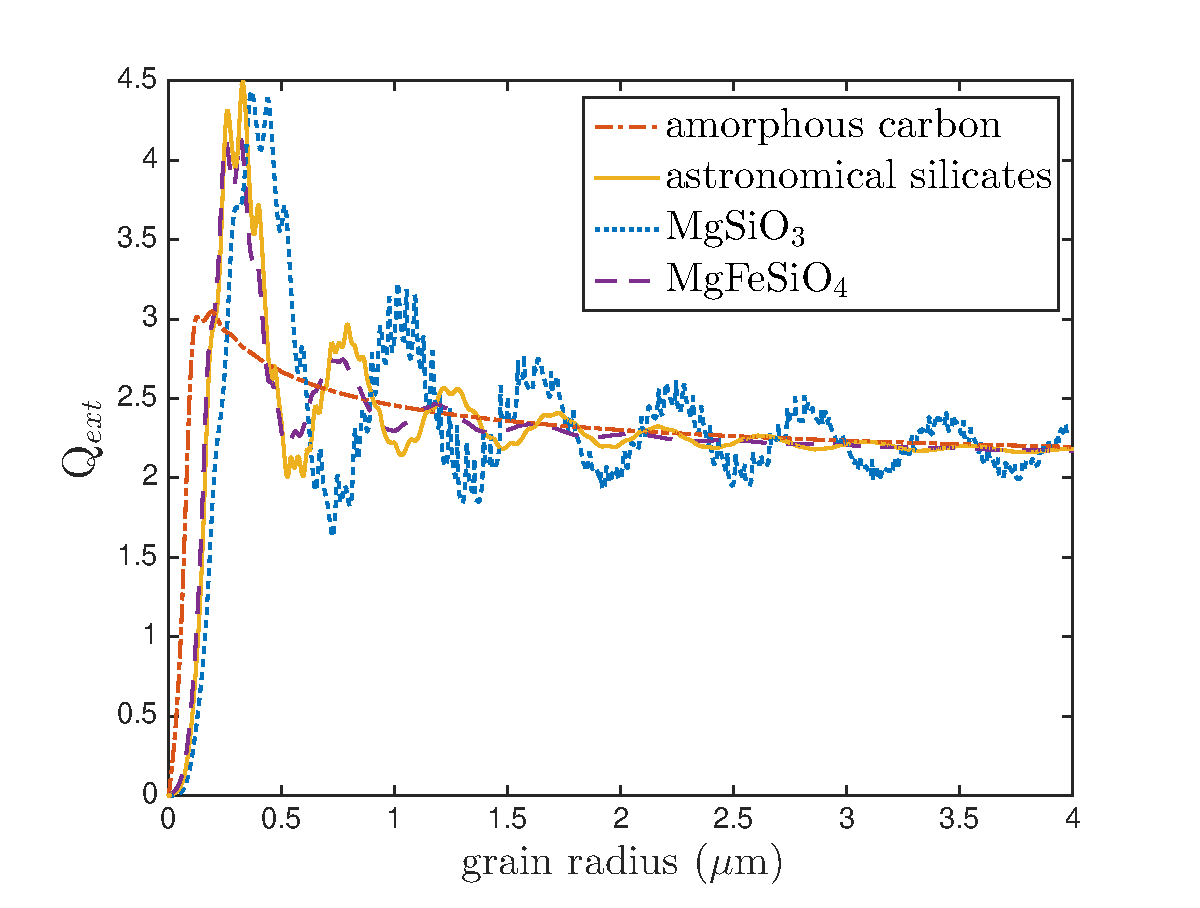
\includegraphics[trim =37 10 45 15,clip=true,scale=0.75]{chapters/chapter4/images/Qext_grainsize_upto4}
\end{subfigure}\\[1ex]
\begin{subfigure}{\textwidth}
\centering
\includegraphics[trim =35 10 45 15,clip=true,scale=0.75]{chapters/chapter4/images/Qext_grainsize_upto4_log}
\end{subfigure}
\caption{Variation of extinction efficiency ($Q_{ext}$) with grain size for amorphous carbon and silicates using Mie theory at $\lambda = 658 \mu $m. Optical constants are from \citet{Zubko1996} and \citet{Draine1984}. A linear scale is presented on the top and a log scale on the bottom.}
\label{Qext_grain}
\end{figure}

\begin{figure}
\begin{subfigure}{1\textwidth}
\centering
\includegraphics[trim =37 10 45 15,clip=true,scale=0.75]{chapters/chapter4/images/albedo_grainsize_upto4}
\end{subfigure}\\[1ex]
\begin{subfigure}{1\textwidth}
\centering
\includegraphics[trim =35 10 45 15,clip=true,scale=0.75]{chapters/chapter4/images/albedo_grainsize_upto4_log}
\end{subfigure}
\caption{Variation of albedo with grain size for amorphous carbon and silicates using Mie theory at $\lambda = 658 \mu $m. Optical constants are from \citet{Zubko1996} and \citet{Draine1984}. A linear scale is presented on the top and a log scale on the bottom.}
\label{albedo_grain}
\end{figure}

The dependence of the shape of the line profile in the optically thin dust case 
is described in Section \ref{analytics}.  However, the density profile 
also plays a significant role where there is even a small amount of 
absorption.  As previously discussed, at relatively small optical depths, 
a section of the flat-topped region is removed resulting in a peak at 
$-V_{min}$.  The shape of the profile in this region is significantly 
affected by the density profile.  Shallow density profiles (low $\beta$) produce a virtually 
linear variation in flux between $-V_{min}$ and $+V_{min}$.  For a fixed dust
optical depth, the steeper the distribution becomes, the more concave the 
profile becomes between $-V_{min}$ and $+V_{min}$, ultimately resulting in 
a clear shoulder to the profile at $+V_{min}$.  For extremely steep density
distributions this can result in a double peaked profile with 
trough to the red of $V=0$.  A illustration of the effects of variation of 
$\beta$ with $\tau$ on the profiles is shown in Figure \ref{bt}.

\subsection{Inferring properties of the dust from the models}

The presence of an extended red wing at large positive velocities in 
combination with increased extinction on the red side at smaller positive 
velocities can allow the values of $\tau$ and $\omega$ to be well 
constrained.  In this case it is possible to translate these values into a 
dust mass and average grain size respectively for a given species or combination of 
species using  optical properties and Mie theory (see Figures 
\ref{Qext_grain} and \ref{albedo_grain}).  In fact, it is the dust mass and average grain size 
that is varied within the code for a specified species or combination of 
species i.e. the dust optical depth and grain size are not varied directly.  It is therefore important to note that the use of different 
optical properties may substantially alter the inferred optical depths and 
albedos for a given species of specific grain size as has been noted 
previously (e.g. \citet{Owen2015}).



For amorphous carbon, the larger the grain size used the larger the albedo 
and the smaller the cross-section of absorption.  Larger masses of dust 
are therefore required to fit the same degree of absorption if a larger 
grain size is used.  This is in contrast to SED radiative transfer 
modelling where larger grain sizes generally result in less dust being 
required to fit the IR portion of the SED (W15).  These two techniques in 
tandem may therefore give excellent limits on grain sizes for different 
species or combinations thereof.

\begin{figure}
\begin{subfigure}{0.5\textwidth}
\includegraphics[trim =30 31 45 0,clip=true,scale=0.45]{chapters/chapter4/images/dustdep/a0_001_opt_thin_HaHbPad}
\end{subfigure}
\hspace{4mm}
\begin{subfigure}{0.5\textwidth}
\includegraphics[trim =59 31 45 0,clip=true,scale=0.45]{chapters/chapter4/images/dustdep/a0_001_opt_thick_HaHbPad}
\end{subfigure} \\[1ex]

\begin{subfigure}{0.5\textwidth}

\includegraphics[trim =30 31 45 0,clip=true,scale=0.45]{chapters/chapter4/images/dustdep/a0_1_opt_thin_HaHbPad}
\end{subfigure}
\hspace{4mm}
\begin{subfigure}{0.5\textwidth}
\includegraphics[trim =59 31 45 0,clip=true,scale=0.45]{chapters/chapter4/images/dustdep/a0_1_opt_thick_HaHbPad}
\end{subfigure} \\[1ex]

\begin{subfigure}{0.5\textwidth}
\includegraphics[trim =30 0 45 15,clip=true,scale=0.45]{chapters/chapter4/images/dustdep/a1_opt_thin_HaHbPad}
\end{subfigure}
\hspace{3mm}
\begin{subfigure}{0.5\textwidth}
\includegraphics[trim =51 0 45 15,clip=true,scale=0.45]{chapters/chapter4/images/dustdep/a1_opt_thick_HaHbPad}
\end{subfigure}
\caption{Model line profiles for H$\alpha$ (6563\AA\ in red), H$\beta$ (4861\AA\ in yellow) and Pa$\delta$ (10049\AA\ in blue) for optically thin and  optically thick cases on the left-hand side and right-hand side respectively.  All models adopted density profile $\rho(r) \propto r^{-4}$ (i.e. $\beta = 2$), velocity profiles $v(r) \propto r$ and radii ratio $R_{in}/R_{out}=0.2$.  The grain radii used were $a=0.001~\mu$m (top), $a=0.1~\mu$m (middle) and $a=1.0~\mu$m (bottom). All the above models used amorphous carbon.}
\label{wav_dep}
\end{figure}

\begin{figure}
\begin{subfigure}{\textwidth}
\centering
\includegraphics[trim =30 30 45 25,clip=true,scale=0.55]{chapters/chapter4/images/Qabs_a0_001}
\end{subfigure} \\[0.5ex]

\begin{subfigure}{\textwidth}
\centering

\includegraphics[trim =30 30 45 25,clip=true,scale=0.55]{chapters/chapter4/images/Qabs_a0_1} 
\end{subfigure} \\[0.5ex]

\begin{subfigure}{\textwidth}
\centering
\includegraphics[trim =30 10 45 25,clip=true,scale=0.55]{chapters/chapter4/images/Qabs_a1_0}
\end{subfigure}
\caption{The variation of amorphous carbon dust absorption efficiency with grain size. The grain radii plotted are $a=0.001~\mu$m (top), $a=0.1~\mu$m (middle) and $a=1.0~\mu$m (bottom).  The vertical lines mark the wavelengths of H$\alpha$ (6563\AA\ in red), H$\beta$ (4861\AA\ in yellow) and Pa$\delta$ (10049\AA\ in blue).}
\label{wav_dep2}
\end{figure}






\subsection{Observable signatures of dust in line profiles}
\label{asym}

The greater the dust optical depth, the more attenuation of the line 
is observed.  As expected, the red side of the profile suffers a greater 
degree of absorption than the blue side.  The resulting asymmetry is 
somewhat more complex than perhaps previously thought however.  Dust has 
repeatedly been cited as the agent responsible for the apparent 
blue-shifting of line profiles in supernovae in the manner of the profiles 
presented in Figure \ref{fig:Lucy}.  That is, relatively high optical 
depths result in an overall shift of the entire profile towards the blue.

In practice a relatively large optical depth ($\tau \approx 2$) is 
required to actively shift the peak of the profile bluewards of its natural 
$V_{min}$ value corresponding to the velocity at the inner radius of the shell.  In most cases it seems more likely that the dust
may not be optically thick and the blue-shifting of the peak of the profile is 
likely a result of attenuation in the flat-topped section (close to 
$R_{in}$).  The peak would therefore tend to be located at $-V_{min}$.

Since dust absorption is wavelength dependent for $2\pi a < \lambda$, one might expect the 
position of the peak flux to be dependent on the wavelength of the line being 
considered.  The relationship between the locations of the peaks 
of profiles and their wavelength has been discussed by several authors in 
relation to dust formation \citep{Smith2012, Fransson2013, Gall2014}.  Whilst this may occur in cases of high dust 
optical depth, this is not necessarily likely to be seen in the ejecta of 
most supernovae.  The wavelength-dependence of dust absorption instead 
can result in differing degrees of extinction in the flat-topped region of 
each profile but still leave the peak at its blue-shifted position of 
$-V_{min}$.  Of course, the value of $V_{min}$ may be different for 
different species.  However, if this is the case then there would be no 
reason to expect a variation in the position of the peak of profiles to be 
correlated with the wavelength dependence of dust.  Rather one would 
expect it potentially to trace the location of different ions within the ejecta. 
However, for lines from the same ion, for example the Balmer and Paschen lines of HI,
I might expect to see peaks at the same position but differing degrees of absorption.
At high resolutions, it might be possible to detect differences in the shape of the line 
profiles, particularly between $-V_{min}$ and $+V_{min}$ where the steepness of the 
incline traces the degree of dust absorption.  This can be seen in Figure \ref{wav_dep} 
where I illustrate the effects of the wavelength dependence of dust absorption for 
three lines, H$\alpha$ (6563\AA), H$\beta$ (4861\AA) and Pa$\delta$ (10049\AA).  
All lines were modelled using three different grain sizes and in both optically thin and 
thick cases.  I also show the variation of the absorption cross-section with 
wavelength at three different grain sizes in Figure \ref{wav_dep2}.

The attenuation of the flat-topped region is  often such that it can 
be hard to discern a difference in slope between the attenuated 
section between $-V_{min}$ and $+V_{min}$ and the slope of the wing for 
$V>+V_{min}$, particularly in circumstances where data is of poor 
resolution or has a poor signal-to-noise ratio.  Even in the case of 
excellent data, it may be easy to overlook these particular features or to 
dismiss them as natural fluctuations in the geometry of the ejecta rather than 
that they may be a product of dust absorption effects.

The greater attenuation of radiation received from the receding portion of 
the ejecta results in an asymmetry of the line profile whereby the 
majority of the observed emission is located bluewards of the peak.  
However, the effects of repeated dust scattering events within the 
ejecta can serve to counter this asymmetry.  Even in the case of dust grains 
with a relatively low albedo, a surprisingly persistent wing on the red 
side of the profile is seen beyond the maximum theoretical velocity 
of the emitting region.  For higher albedos this can actively result in a 
shift in the overall asymmetry of the profile, with the majority of the 
emission being emitted redwards of the peak, though the peak itself 
remains blue-shifted.

This effect is obviously analogous to that of electron scattering which 
also produces a significant red wing in line profiles \citep{Hillier1991, 
Auer1972}. This is an important consideration in both modelling and 
analysis of spectral line profiles.  DAMOCLES has the capacity to include 
a basic electron scattering mechanism in order to assess the possibility 
that any observed red wing might be produced by electron scattering rather 
than dust scattering.  The red wing observed in line profiles is an 
excellent diagnostic for determining the overall dust albedo and it is 
therefore important to establish whether this feature is due to 
electron or dust scattering or a combination of the two.

The combination of relatively low optical depths, initially flat-topped 
profiles, greater attenuation on the blue side with increased flux on the 
red side due to scattering can result in a profile that ends up appearing 
almost symmetrical, particularly if 
contaminants, such as narrow lines or blending with other broad lines, are 
present or if the resolution of the data is low.  The potential for apparently 
symmetrical profiles that appear to have been uniformly blue-shifted 
should be noted (see Figures \ref{bt} and \ref{wt} for examples of this).



\subsection{The effect of a grain size distribution}
\label{gs_distn}
It is important to consider the potential effect on the dust mass of modelling a grain size distribution instead of a single grain size.  For a grain size distribution the overall extinction cross section, $C_{ext}$, at a given wavelength is calculated as

\begin{equation}
C_{ext}=\int^{a_{max}}_{a_{min}} Q_{ext}(a) n(a) \pi a^2 da 
\end{equation}

where $Q_{ext}(a)$ is the extinction efficiency for a grain size $a$ and $n(a)$ is the number of grains with size $a$. The overall extinction efficiency is then

\begin{equation} 
Q_{ext} = \frac{C_{ext}}{ \int^{a_{max}}_{a_{min}} n(a) \pi a^2 da} 
\end{equation}
 
The scattering cross-section $Q_{sca}$ is similarly calculated.  As a result of these calculations, there is rarely a single grain size that has the same albedo and extinction efficiency as a size distribution.  Modelling a size distribution instead of a single grain size may therefore alter the deduced dust mass.  Since models are only sensitive to the optical depth and the albedo, however, it is not possible to deduce the grain size range or distribution and only single grain sizes are investigated in the models that are presented in the following chapters.

Whilst this apparently limits the scope of these results, it is important to consider the extent to which considering grain size distributions would alter the derived dust masses.  By considering a number of grain size ranges and adopting a power law distribution with a variable exponent, I may gain some insight into the effects of adopting a distribution rather than a single size.  For the classical MRN power law ($n(a) \propto a^{-3.5}$) with a wide grain size range ($a_{min} = 0.001 \mu$m to $a_{max} = 4.0 \mu$m) the derived albedo of $\omega=0.001$ is much too small to reproduce the required wing seen at early epochs.  I investigate this issue by adjusting the exponent of a distribution for a number of grain size ranges until the overall albedo is the same as that seen for the best fitting single grain size.  I can then approximately calculate the required dust mass for a distribution of grain sizes from the properties of a single-size model by equating the optical depths.  The optical depth for a single grain size is proportional to 

\begin{equation}
\tau \propto Q_{ext}(a)  \sigma(a) n_d
\end{equation}

\noindent where $n_d$ is the number density of dust grains, $\sigma(a)$ is the cross-sectional area of a grain of radius $a$ and $Q_{ext}(a)$ is the extinction efficiency for a grain of radius $a$.  On average, this gives

\begin{equation}
\tau \propto \frac{Q_{ext}(a) M \pi a^2}{\frac{4}{3} \pi a^3 \rho V}
\end{equation}

\noindent for a total dust mass $M$, total volume of the ejecta $V$ and density of a dust grain $\rho$.

This simplifies to 

\begin{equation}
\tau \propto \frac{Q_{ext}(a) M}{\frac{4}{3} a \rho V}
\end{equation}

\begin{equation}
\label{distn_conv}
M_{d}= \frac{M_s Q_{ext,s}(a_s)}{a_s} \times \frac{\int^{a_{max}}_{a_{min}} n(a) a^3 da}{\int^{a_{max}}_{a_{min}} Q_{ext}(a) n(a) a^2 da}
\end{equation}

where the subscript $s$ represents the single grain size quantities and the subscript  $d$ represents quantities for the grain size distribution.  This is only calculable for a specific wavelength and is therefore only an approximate conversion when performed at the rest-frame wavelength of the line in question.  However, practically, the variation of extinction efficiency and albedo over the narrow wavelength ranges modelled within the code is not significant and so this method produces relatively accurate dust masses (as determined by running models with the new parameters).

\subsection{The effect of different species}

In the majority of the modelling that follows, a single species, amorphous carbon, is considered.   A single species is used since the parameters that affect the quantity of dust required in the model are the albedo and the optical depth.  There are therefore  likely many possible combinations of species that may result in a good fit to the data.  The choice of amorphous carbon is partly motivated by evidence that, for SN~1987A (which, as an incredibly well-observed and relatively typical core-collapse supernova, is an excellent test case) the fraction of silicates present in the dusty ejecta is limited to approximately 15\% (W15, \citet{Ercolano2007}).  It is also motivated by previously published SED models which generally employ amorphous carbon.  This is because SED models frequently require far larger masses of silicate dust than amorphous carbon dust in order to produce similar levels of infrared flux and therefore amorphous carbon models are likely to produce the more conservative dust mass estimates.  By modelling with amorphous carbon I may compare directly to these models where possible.

I consider the change in dust mass when a medium of 100\% silicates is used instead of amorphous carbon.  I use optical constants presented in \cite{Draine1984}.  In a similar manner to the approach detailed in Section \ref{gs_distn}, I may calculate the mass of silicates that is equivalent to a carbon mass for a single grain size.  I consider the albedo at the original grain size, calculate the equivalent grain size for silicates that results in the same albedo and then calculate the new dust mass by considering the change in the extinction efficiency as

\begin{equation}
M_{sil} = M_{amc} \Big( \frac{Q_{amc}}{Q_{sil}} \Big) \Big(\frac{a_{sil}}{a_{amc}}\Big) \Big(\frac{\rho_{sil}}{\rho_{amC}}\Big)
\end{equation}

Because of the nature of the variation of albedo with grain size for silicates (see Figure \ref{albedo_grain}), there is often more than one silicate grain size that will give rise to the same albedo.  I consider all the possibilities and the resulting mass conversion factors in Table \ref{tb_sil}.  In my best fitting models for days 714 and 806, using any fraction of silicates of either grain size would serve to increase the dust mass.  However, at later epochs, using some fraction of silicate dust would reduce the dust mass to potentially more than half of my estimated values. However, this is still within my predicted range and my minimum and maximum dust masses remain robust.

\begin{table}
	%\begin{minipage}{180mm}
	\caption{Equivalent dust masses for the day 714 clumped models using grain size distributions and 100\% amorphous carbon. $f$ is factor of increase from the dust mass for the single size model ($M=7 \times 10^{-5} M_{\odot}$ with $a=0.6 \mu$m) and $p$ is the exponent of the grain size distribution $n(a) \propto a^{-p}$.}
	\label{tb_sil}
	\begin{center}
  	\begin{tabular}{@{} cccccc @{}}
    	\hline
	\multicolumn{2}{c}{\textit{carbon}} && \multicolumn{2}{c}{\textit{silicates}} & \\
$a$ & $Q_{ext}$ & &$a$& $Q_{ext}$ & $f=M_{sil}/M_{amc}$ \\
\hline
0.6 & 2.60633 & &0.0583 & 0.0772 & 5.37 \\
0.6 & 2.60633 & &4 & 2.1828 & 13 \\
 \\
3.5 & 2.2129 & &0.0641 & 0.10182 & 0.65 \\
3.5 & 2.2129 & &1.02 & 2.149 & 0.49 \\
3.5 & 2.2129 & &1.376 & 2.3514 & 0.61 \\


    \hline
  \end{tabular}
  \end{center}
%\end{minipage}
\end{table}

\subsection{The velocity distribution}
\label{scn:vel_prof}








